% !TeX document-id = {3c9fb181-ef8d-46f4-a369-f483876e4c37}
% !TeX TXS-program:compile = txs:///pdflatex/[--shell-escape]


\documentclass[fleqn,11pt,aspectratio=169]{beamer}
\usepackage{tubslogo}
\usepackage{amsmath}
\usepackage{amsfonts}
\usepackage{amssymb}
\usepackage{graphicx}
\usepackage{qrcode}
\usepackage{geometry}
\usepackage{tikz}
\usepackage{amsthm}
\usepackage{float}
\usepackage{cleveref}
\usepackage{acronym}
\usepackage{algpseudocode}

\usepackage{fancyvrb}
\usepackage{fvextra}
\usepackage[normalem]{ulem}
\usepackage{enumerate}

\usepackage[overload]{textcase}
\usepackage{minitoc}        
%\usepackage{etoc}        
\usepackage{printlen}
\usepackage{url}  
\usepackage{tabularx}  
\usepackage{soul}
\usepackage{siunitx}
\usepackage{eqparbox}
\sisetup{
	per-mode=symbol,
}
\usepackage[utf8]{inputenc}
\usepackage[
	backend=biber,
	style=numeric,
]{biblatex}

\usepackage[rgb,dvipsnames]{xcolor}

\selectcolormodel{natural}
\usepackage{ninecolors}
\selectcolormodel{rgb}
\usepackage{tabularray}
\usepackage{minted}
\usemintedstyle{emacs,tabsize=2,linenos,xleftmargin=10pt,highlightcolor=cyan}

\usepackage[export]{adjustbox}% http://ctan.org/pkg/adjustbox

\usepackage[append]{beamersubframe}
\usepackage[american]{babel}
\usepackage{graphicx}
\setbeamerfont{normal text}{size=12pt}

\date{June 04, 2026}
\usetheme[%
  %nexus,%        Nexus Fonts benutzen
  %lnum,%         Versalziffern verwenden
  %cmyk,%<rgbprint>,          Auswahl des Farbmodells
  blue,%<orange/green/violet> Auswahl des Sekundärfarbklangs
  dark,%<light,medium>        Auswahl der Helligkeit
  %colorhead,%    Farbig hinterlegte Kopfleiste
  %colorfoot,%    Farbig hinterlegt Fußleiste auf Titelseite
  colorblocks,%   Blöcke Farbig hinterlegen
  %nopagenum,%    Keine Seitennumer in Fußzeile
  %nodate,%       Kein Datum in Fußleiste
  tocinheader,%   Inhaltsverzeichnis in Kopfleiste
  %tinytocinheader,% kleines Kopfleisten-Inhaltsverzeichnis
  %widetoc,%      breites Kopfleisten-Inhaltsverzeichnis
  %narrowtoc,%    schmales Kopfleisten-Inhaltsverzeichnis
  %nosubsectionsinheader,%  Keine subsections im Kopfleisten-Inhaltsverzeichnis
  %nologoinfoot,% Kein Logo im Fußbereich darstellen
  ]{tubs}
% Titelseite
%\title{towards TPU: A Survey into Accelerators for Cloud AI}
\title{Algorithm Engineering 2026: Sheet 03}
\author{Rouven Kniep}

%titlepage font and background
\setbeamercolor{titlebarfirst}{parent=titlepage, bg=titlepage.bg!0}

% Edit the TUBS template to move the tubslogo into place for the title
\let\tubslogoAbsOld\tubslogoAbs
\renewcommand{\tubslogoAbs}[1]{\raisebox{-2.3mm}{\tubslogoAbsOld{#1}}}

% Quoteblock 
\newcommand{\quotebox}[1]{\begin{center}\fcolorbox{white}{blue!15!gray!15}{\begin{minipage}{0.9\linewidth}\vspace{10pt}\center\begin{minipage}{0.8\linewidth}{\space\Huge``}{#1}{\hspace{1.5em}\break\null\Huge\hfill''}\end{minipage}\smallbreak\end{minipage}}\end{center}}



\begin{document}

\part{main}
\begin{frame}[plain]
	\titlepage
\end{frame}	

\begin{frame}{evaluation}
	\begin{center}
		\qrcode[height=0.6\textheight]{https://umfragen.tu-bs.de/evasys/online.php?pswd=9728N}
		
		\vspace{15pt}
		
		\url{https://umfragen.tu-bs.de/evasys/online.php?pswd=9728N}
	\end{center}
	
\end{frame}


\section{Ex1}

\begin{frame}{Ex1: Setting}
	\begin{center}
		Mutually Exclusive Knapsack
	\end{center}
	\begin{columns}[T]
		\column{0.3\textwidth}
		Given: Instance with¨
		\begin{itemize}
			\item Items $X = \{x_1,\dots,x_n\}$
			\item Profits $p_i \in \mathbb{R}_{\geq0}$
			\item Weights $w_i \in \mathbb{R}_{\geq0}$
			\item Capacity $c \in \mathbb{R}_{\geq0}$
			\item Excluded items $E_i \subseteq X$ (symmetrical)
		\end{itemize}
		\column{0.5\textwidth}
		Constraints and Target
		\begin{itemize}
			\item find solution $S \subseteq X$ with:
			\item $max \sum_{i=1}^{n} p_i*x_i$ \\(optimization function), subject to:
			\item $\sum_{i=1}^{n} w_ix_i \leq c$ (within capacity)
			\item $\forall i: \forall j\in E_i: x_i+x_j \leq 1$ \\(mutually exclusive)
			\item $\forall i: x_i \in \mathcal{B} = \{0;1\}$ (binary variables)
		\end{itemize}
	\end{columns}
\end{frame}

\begin{frame}{Ex1a: Constraint Propagation (overview)}
	\begin{columns}
		\column{0.47\textwidth}
		{ \large Terminology}
		
		\begin{tblr}{colspec={c|X|X}}
		what? & best found solution & best possible value \\
		validity & global & local (node) \\
		\hline
		min. & upper bound & lower bound \\
		max. & lower bound & upper bound \\
		\hline
		Gurobi & incumbent & bound \\
		CP-SAT & objective & bound \\
		\end{tblr}
		
		\column{0.47\textwidth}
		In each node:
		\begin{enumerate}
			\item dequeue node
			\item if incumbent $\geq$ bound: next node
			\item \textbf{constraint propagation} - extend node's partial solution
			\item get bound + improve bound with cuts
			\item update stats
			\item if incumbent $\geq$ bound: next node
			\item otherwise: generate + enqueue branches
		\end{enumerate}
	\end{columns}	
\end{frame}

\begin{frame}{Ex1a: Constraint Propagation}
	
\begin{center}
	\large given: partial assignments $P$: \texttt{list[bool|None]}
\end{center}

\hrule

\vspace{5pt}
constraints: mutually exclusive - w.l.o.g. let $x_i + x_j \leq 1$ and $P_i \in$ \texttt{bool}
\begin{itemize}
	\item if $P_i$=\texttt{False}: constraint unnecessary
	\item if $P_i$=\texttt{True}: boolean case: $\implies P_j$ = \texttt{False}; fractional case: $\implies x_j^* = 0$
	\item $\implies$ no gain to be had
\end{itemize}

\hrule

\vspace{5pt}
constraint: capacity $\sum_{i=1}^{n} w_ix_i \leq c$  
\begin{itemize}
	\item let $rem = c - \sum_{i=1}^{n}(w_i \mid P_i =$ \texttt{False}$)$
	\item w.l.o.g let $\exists j \mid w_j < rem$
	\item boolean case: $\implies P_j$=\texttt{False}
	\item fractional case: $\implies x_j^* \in [0;1)$
	\item $\implies$ relaxation may assume impossible values $\implies$ propagate! 
\end{itemize}
\end{frame}

\begin{frame}[fragile]{Ex1a: Constraint Propagation (solution)}
\begin{minted}{python}
def constraint_propagation(self, partial_assignment: list[bool | None]):
	remaining_capacity = self.instance.capacity = sum(
		self.index_to_item[i].weight
		for i, assigned in enumerate(partial_assignment)
		if assigned
	)
	for i, assigned in enumerate(partial_assignment):
		if assigned is None:
			if self.index_to_item[i].weight > remaining_capacity:
				partial_assignment[i] = False
\end{minted}
\end{frame}


\begin{frame}[t, fragile]{Ex1a: Constraint Propagation (wrong solution)}

\begin{minted}{python}
def constraint_propagation(self, partial_assignment: list[bool | None]):
	remaining_capacity = self.instance.capacity
	for i, assigned in enumerate(partial_assignment)
		if assigned is None:
			if self.index_to_item[i].weight >= remaining_capacity:
				partial_assignment[i] = False
		elif assigned is True:
			remaining_capacity -= self.index_to_item[i].weight
\end{minted}

\only<1>{
}
\only<2>{
\begin{itemize}
	\item wrong comparison (ln. 5): would disable fitting items \\
	$\implies$ INCORRECT! Algorithm will throw out valid solutions!
	\item merged loops: \texttt{remaining\_capacity} is decreased after propagation check \\
	$\implies$ valid, but too weak: does not disable all eligible items  
\end{itemize}
}
\end{frame}

\begin{frame}[fragile]{Ex1b: Heuristic}
\begin{minted}{python}
for rd in range(ROUNDS): # ROUNDS = 1000 - still 0.1s!
	result = [False] * len(self.instance.items)
	candidates = sorted_idxs.copy(); excludes = set()
	profit = 0.0; remaining_cap = self.instance.capacity
	while candidates:
		num_choices = min(len(candidates), NUM_CANDIDATES)
		i = random.choice(candidates[:num_choices])
		candidates.remove(i); item = self.item_to_index[i]
		if item.weight <= remaining_cap and item.name not in excludes:
			remaining_cap -= item.weight; profit += item.profit
			result[i] = True; excludes.update(item.excludes)
	if profit > best_profit:
		best_profit = profit; best_result = result
\end{minted}
\end{frame}

\begin{frame}{Ex1c: Knapsack Cuts}
	\begin{columns}
		\column{0.4\textwidth}
		Flow:
		\begin{enumerate}
			\item calculate relaxation
			\item if relaxation is int: return
			\item if \texttt{cut\_rounds++} $>$ \texttt{max\_cut\_rounds}: return
			\item try to find cuts
			\item if no cuts found: return
			\item add cuts + repeat
		\end{enumerate}
		\column{0.4\textwidth}
		Idea: find $D \in [1;n]$, s.t.
		\begin{enumerate}
			\item $\sum_{i\in D} w_i > c$
			\item $\sum_{x_i^*} > |D|-1$
		\end{enumerate}
	\end{columns} 
\end{frame}

\begin{frame}[fragile]{Ex1c: Knapsack Cuts}
	\begin{minted}{python}        
best_cut_indices = None; best_violation = 0.0
for sorted_indices in (sorted_indices_1, sorted_indices_2):
	weight_sum = 0.0; value_sum = 0.0; cut_indices = []
	for i in sorted_indices:
		weight_sum += self.index_to_item[i].weight
		value_sum += solution[i]; cut_indices.append(i)
		violation = value_sum - (len(cut_indices) - 1) - CUT_VIOLATION_TOLERANCE
		if weight_sum > capacity_with_buffer:
			if violation > best_violation:
				best_violation = violation
				best_cut_indices = cut_indices.copy()
			break
		if violation <= best_violation:
			break
	\end{minted}
\end{frame}

\begin{frame}[t]{Ex1d: Clique Cuts - which items to include}
	\begin{center}
		\only<1>{
		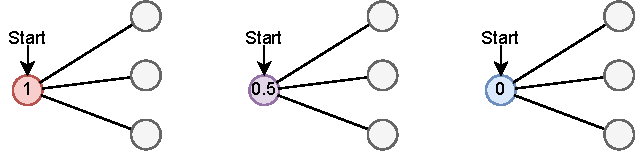
\includegraphics[keepaspectratio, page=1, width=0.9\textwidth]{clique_cut.pdf} }
		\only<2>{
		\includegraphics[keepaspectratio, page=2, width=0.9\textwidth]{clique_cut.pdf} }
	\end{center}
	\begin{columns}
		\only<2>{
		\column{0.3\textwidth}
		all candidates have value 0
		$\implies$ no cuts
		\column{0.3\textwidth}
		candidates have values 0-0.5
		$\implies$ interesting!
		\column{0.3\textwidth}
		unlikely (interesting cliques found from 2.)
		}
	\end{columns} 
\end{frame}

\begin{frame}[t]{Ex1d: Clique Cuts - Clique Size}
	\begin{columns}
		\column{0.4\textwidth}
		\includegraphics[keepaspectratio, page=3, width=\textwidth]{clique_cut.pdf}
		\column{0.4\textwidth}
		\begin{itemize}
			\item avoid items of value 1
			\item maximum clique constraints imply all smaller ones:\\
				\textcolor{Purple}{$x_1^*+x_2^*+x_3^*+x_4^*$}$+$\textcolor{Dandelion}{$x_5^*$}$\leq1$
				$\implies$\textcolor{Purple}{$x_1^*+x_2^*+x_3^*+x_4^*$}$\leq1$
		\end{itemize}
	\end{columns} 
\end{frame}

\begin{frame}[fragile]{Ex1d: Clique Cuts}
	\begin{minted}{python}        
def clique_cut_separation(self, solution: Sequence[float]) -> list[int] | None:
	sol = list(solution)
	candidates = [i for i, value in enumerate(sol)
		if (value > INTEGRALITY_TOLERANCE
		and value < 1 - INTEGRALITY_TOLERANCE)]
	candidates.sort(key=lambda i: sol[i], reverse=True)
	best_clique: list[int] = []; best_value = 0.0
	# inner loop, see next slide
	if best_value <= 1.0 + CUT_VIOLATION_TOLERANCE:
		return None
	else: 
		return best_clique
	\end{minted}
\end{frame}


\begin{frame}[fragile]{Ex1d: Clique Cuts}
	\begin{minted}{python}
	# candidates are without 1 and 0 -> all are interesting        
	for anchor in candidates[:20]:
		clique = [anchor]; value = solution[anchor]
		extensions = self.exclusion_graph[anchor].copy()
		while extensions:
			best = min(extensions, key=lambda i: solution[i])
			clique.append(best); value += solution[best]
			extensions.intersection_update(self.exclusion_graph[best])
		if value > best_value:
			best_value = value; best_clique = clique.copy()
	\end{minted}
\end{frame}

\section{Ex2}
\begin{frame}{Ex2: Exam Scheduling - Setting}
	\begin{center}
		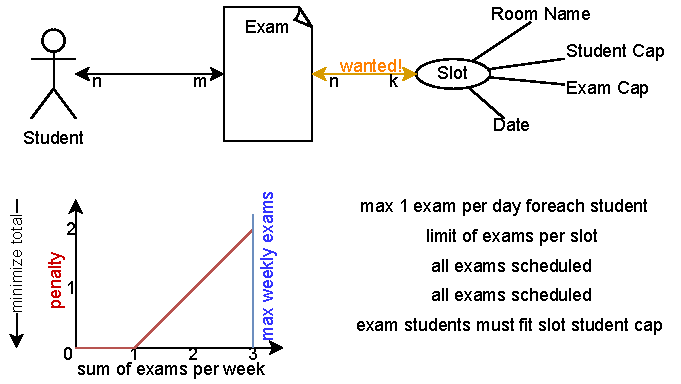
\includegraphics[page=1, keepaspectratio, width=\textwidth, height=0.9\textheight]{examscheduling.pdf}
	\end{center}
\end{frame}

\begin{frame}[fragile]{Variables per Sitting? (wrong!)}
	\begin{columns}
		\column{0.6\textwidth}
	\begin{minted}{python}
 def _make_vars(self):
	self.vars = {
		(exam, slot, sitting): 
		self.model.new_bool_var(
			name=f"({exam},{slot},{sitting})"
		)
		for exam in self.exams
		for slot in self.instance.slots
		for sitting in range(slot.max_exams)
	}
	\end{minted}
		\column{0.4\textwidth}
		\begin{itemize}
			\item Idea: assign each sub-slot in exams per day individually
			\item so: morning/noon/afternoon/evening...
			\item but: not necessary (we don't need the exact sub-slot for anything)
		\end{itemize}
	\end{columns}
\end{frame}


\begin{frame}[fragile]{Exam-Slot-Variables (good!)}
	\begin{columns}
		\column{0.5\textwidth}
		\begin{minted}{python}
def _make_vars(self):
self.vars = {
	(exam, slot): 
	self.model.new_bool_var(
	name=f"({exam},{slot})"
	)
	for exam in self.exams
	for slot in self.instance.slots
}
		\end{minted}
		\column{0.5\textwidth}
		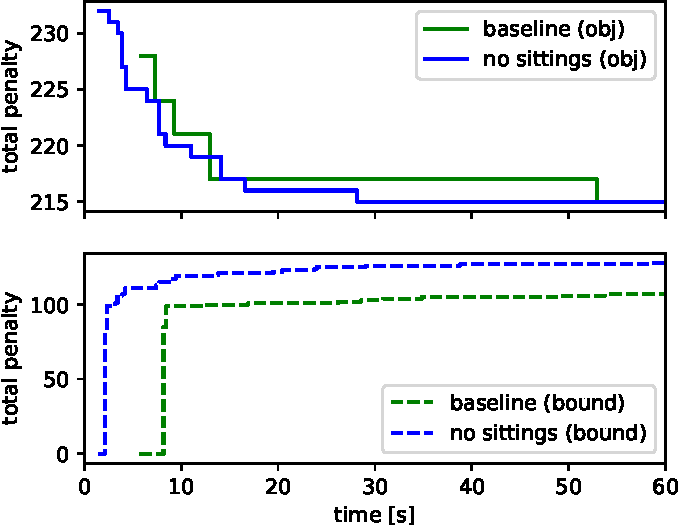
\includegraphics[keepaspectratio, scale=0.6]{2_1.pdf}
		$\implies$ only model needed complexity
	\end{columns}
\end{frame}


\begin{frame}[fragile]{Objective}
	\begin{columns}
		\column{0.5\textwidth}
		
		\includegraphics[page=2, keepaspectratio, width=0.9\columnwidth]{examscheduling.pdf}
		\begin{itemize}
			\item penalty 0 if sum of exams $\leq 1$, $+1$ for each more
			\item not linear! $\implies$ additional \texttt{penalty}-variables needed
		\end{itemize}
		
		\column{0.5\textwidth}
		
		\begin{minted}{python}
for student, exams in self.students.items():
	for isoweek, slots in self.isoweeks.items():
		penvar = self.model.new_int_var(
			0, 3 - 1, 
			f"pen_{student}_{isoweek}")
		self.model.add_max_equality(
			penvar,	0, sum(
				self.vars[(exam, slot)]
				for exam in exams
				for slot in slots
			)- 1)
			self.penalties.append(penvar)
self.model.minimize(sum(self.penalties))
		\end{minted}
	\end{columns}
\end{frame}

\begin{frame}[fragile]{Objective (improved)}
	\begin{columns}[T]
		\column{0.5\textwidth}
		
		\includegraphics[page=2, keepaspectratio, height=0.5\textheight]{examscheduling.pdf}
		\begin{minted}{python}
self.model.add_max_equality(
	penvar,	0, sum(
	self.vars[(exam, slot)]
	for exam in exams
	for slot in slots
)- 1)
		\end{minted}
		
		\column{0.5\textwidth}
		\includegraphics[page=3, keepaspectratio, height=0.5\textheight]{examscheduling.pdf}
		\begin{minted}{python}
self.model.add(penvar + 1
	>= sum(self.vars[(exam, slot)] 
		for exam in exams 
		for slot in slots)
)
		\end{minted}
		
	\end{columns}
\end{frame}

\begin{frame}{Objective (improved)}
	\begin{columns}[T]
		\column{0.5\textwidth}
		\vspace{\dimexpr-2\parsep-2\parskip\relax} % avoid center top space
		\begin{center}
			\includegraphics[page=2, keepaspectratio, height=0.45\textheight]{examscheduling.pdf}
			\includegraphics[page=3, keepaspectratio, height=0.45\textheight]{examscheduling.pdf}
		\end{center}		
		\column{0.5\textwidth}
		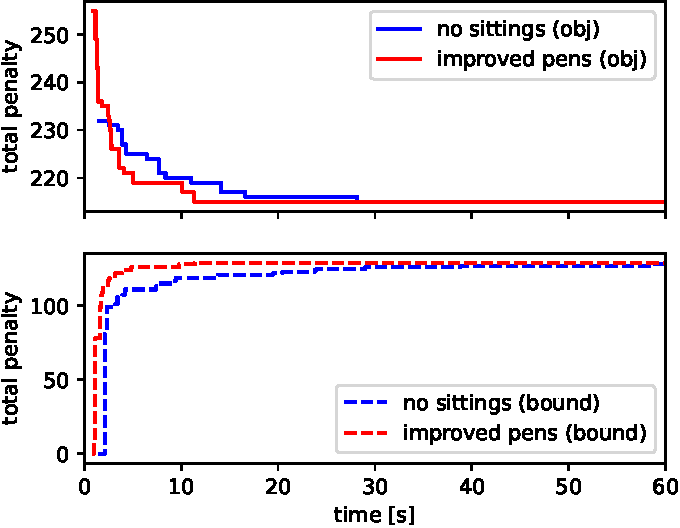
\includegraphics[keepaspectratio, scale=0.6]{2_2.pdf}
		$\implies$ avoid unnecessary non-convex constraints
	\end{columns}
\end{frame}

\begin{frame}[fragile,t]{Room constraints}    
	\begin{minted}{python}
def _exam_constraints(self):
	# Capacity
	for (exam, slot), var in self.vars.items():
		self.model.add(var * self.exams[exam] <= slot.capacity)
	# Held once
	for exam in self.exams:
		self.model.add_exactly_one(
			self.vars[(exam, slot)] for slot in self.instance.slots
		)
	\end{minted}
	\only<2>{
		\begin{itemize}
			\item relaxes poorly: fractional values caused by room cap\\
				(example: 45 cap and 50 students $\implies$ var$\leq0.9$)
			\item room cap and number of students known during model creation\\
				$\implies$ could force variable to 0 or not even make variable
		\end{itemize}}
\end{frame}

\begin{frame}[fragile, t]{Room Constraints (improved)}
	\begin{columns}[T]
		\column{0.5\textwidth}
		\begin{minted}{python}
def _make_vars(self):
	self.vars = {(exam, slot): 
		self.model.new_bool_var(
			name=f"({exam},{slot})")
		for exam, num_students 
			in self.exams.items()
		for slot in self.instance.slots
		if num_students <= slot.capacity
	}
	# and a check that all exams have
	# at least one feasible slot
		\end{minted}
		\column{0.5\textwidth}
		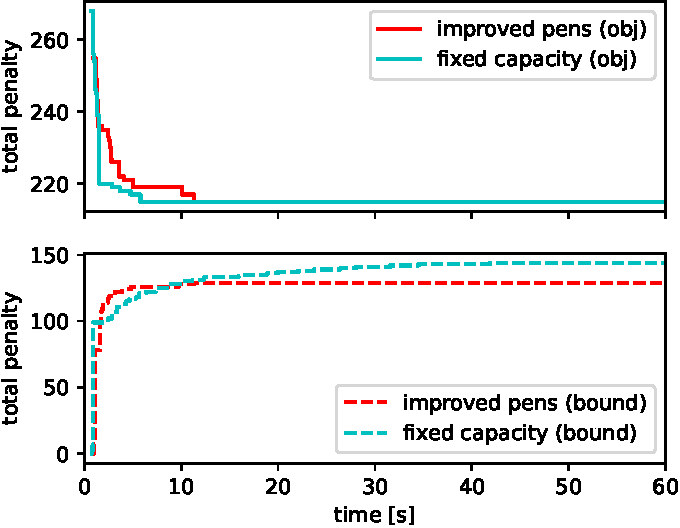
\includegraphics[keepaspectratio, scale=0.6]{2_3.pdf}
		$\implies$ only model constraints and variables about data not known during construction!
	\end{columns}
\end{frame}

\section{Ex3}

\begin{frame}{Exercise 3: Bike Redistribution}
	\begin{columns}
		\column{0.5\textwidth}
		\includegraphics[keepaspectratio, width=\columnwidth]{pickupdelivery.png}
		
		\column{0.4\textwidth}
		\begin{itemize}
			\item bikes: pick up and drop off at locations
			\item vehicle with max capacity
			\item tour from and to depot
			\item distances: given matrix
			\item wanted: shortest tour
		\end{itemize}
	\end{columns}
\end{frame}


\begin{frame}[fragile,t]{Decision Variables}    
	\begin{minted}{python}
def _make_vars(self):
	# arcs: directed edge from node *u* to *v*
	# directed for distance, also performs action at *v*
	self.arc_vars = {
		(u, v): self.model.new_bool_var(f"arc[{u}->{v}]")
		for (u, v) in itertools.permutations(self.all_nodes, 2)
	}	
	# load: loaded bikes after stop at node *n*
	self.load_vars = {
		n: self.model.new_int_var(0, self.instance.capacity, f"load[{n}]")
		for n in self.all_nodes
	}
	\end{minted}
\end{frame}

\begin{frame}[fragile,t]{Objective}
	\begin{minted}{python}
def _objective(self):
	# min total travel distance
	self.model.minimize(
		sum(self.distances[u, v] * lit 
		for (u, v), lit in self.arc_vars.items())
	)
	\end{minted}
	\begin{itemize}
		\item perfectly linear 
		\item no additional helper-variables necessary
		\item good relaxations...
	\end{itemize}
\end{frame}

\begin{frame}[fragile,t]{Capacity Constraints}
	\begin{minted}{python}
def _capacity_link_constraints(self):
	# Channelling: along any used arc (u, v): load[v] = load[u] + delta[v].
	self.model.add(self.load_vars[self.depot] == 0)
	for (u, v), lit in self.arc_vars.items():
		if v == self.depot:
			self.model.add(self.load_vars[u] == 0).only_enforce_if(lit)
		else:
			self.model.add(
				self.load_vars[v] == self.load_vars[u] + self.delta[v]
			).only_enforce_if(lit)
	\end{minted}
	\begin{itemize}
		\item directly based on connection $\implies$ no helpers / no complex implications
	\end{itemize}
\end{frame}

\begin{frame}[fragile,t]{Circuit Constraints (MTZ - Bad)}
\begin{minted}[highlightlines={10,6}]{python}
def _circular_constraint_mtz(self):
	self.order_vars = {n: self.model.new_int_var(
		lb=0, ub=len(self.all_nodes) - 1, name=f"order_{n}")
		for n in self.all_nodes}
	self.model.add(self.order_vars[self.depot] == 0)
	self.model.add_all_different(self.order_vars.values())
	for (u, v), lit in self.arc_vars.items():
		target = len(self.all_nodes) - 1 if v == self.depop
				else self.order_vars[v] - 1
		self.model.add(self.order_vars[u] == target).only_enforce_if(lit) 						
	# + one incoming + one outgoing for every node
\end{minted}
\begin{itemize}
	\item MTZ has a very large (relaxed) polytope
	\item sometimes good with capacity constraints, order numbers, ...
\end{itemize}
\end{frame}

\begin{frame}[fragile,t]{Circuit Constraints (CP-SAT \texttt{add\_circuit})}
\begin{minted}{python}
def _circular_constraint(self):
	self.model.add_circuit([
		(self.node_id[u], self.node_id[v], var)
		for (u, v), var in self.arc_vars.items()
	])
\end{minted}
\begin{itemize}
	\item high-level abstraction
	\item availability and performance depends on solver...
	\item ... if available often VERY good!
\end{itemize}
\end{frame}

\begin{frame}[t]{MTZ vs \texttt{add\_circuit} (no warm-start)}
	\begin{center}
		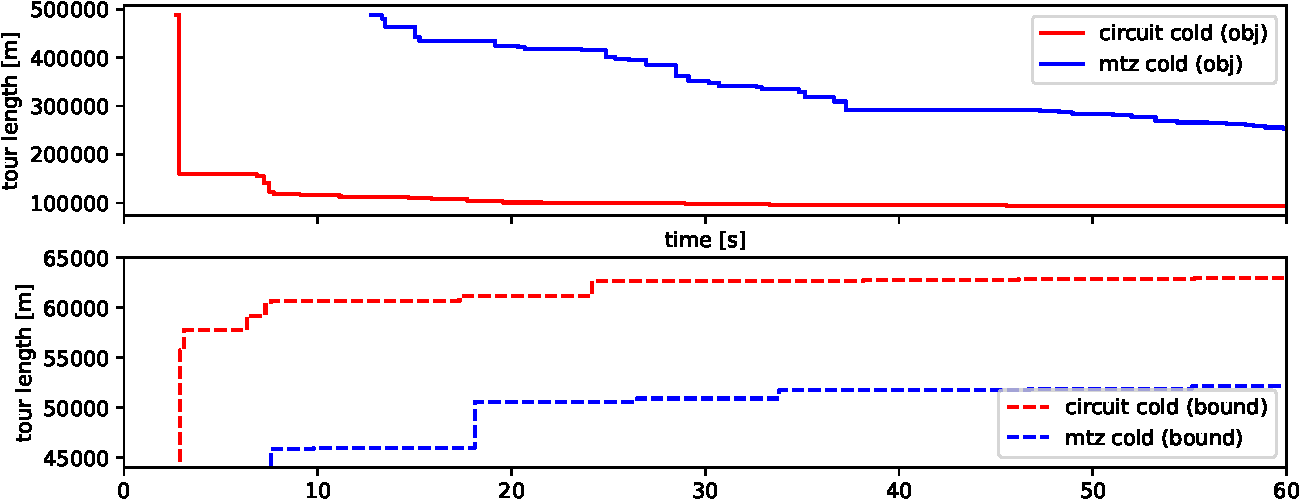
\includegraphics[keepaspectratio, scale=0.6]{3_1.pdf}
	\end{center}
\end{frame}

\begin{frame}[t]{MTZ vs \texttt{add\_circuit} (greedy warm-start)}
	\begin{center}
		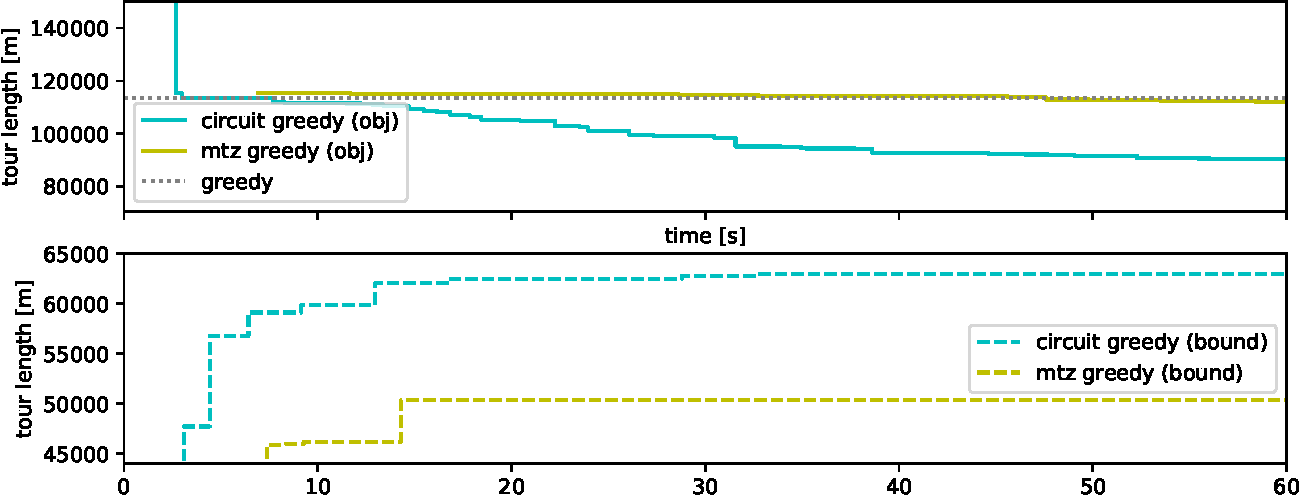
\includegraphics[keepaspectratio, scale=0.6]{3_2.pdf}
		
		a good heuristic can save a bad model, but cannot make a bad model good
	\end{center}
\end{frame}

\begin{frame}[t]{MTZ vs \texttt{add\_circuit} (specialized heuristic warm-start)}
	\begin{center}
		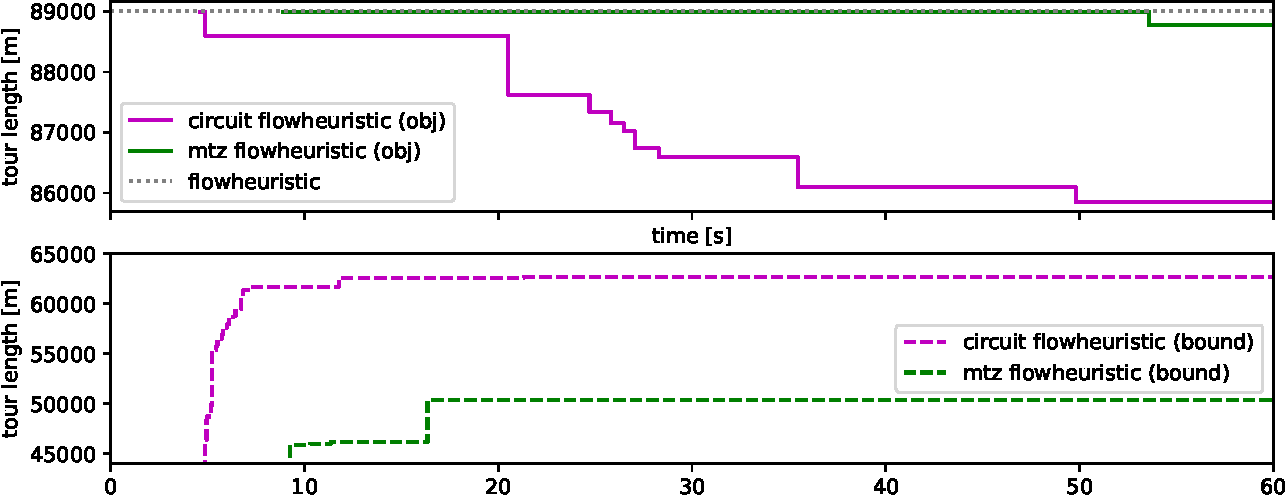
\includegraphics[keepaspectratio, scale=0.6]{3_3.pdf}
		
		a good heuristic can save a bad model, but cannot make a bad model good 
	\end{center}
\end{frame}

\end{document}
